\documentclass[10pt,a4paper]{article}

\usepackage[utf8]{inputenc}
\usepackage{amsmath}
\usepackage{amsfonts}
\usepackage{amssymb}
\usepackage{tikz}
\usepackage{pgf}
\usepackage{pgfplots}
\usepackage{hyperref}
\usepackage{comment}
\usepackage{parskip}

\pgfplotsset{compat=1.3}
\title{Implementation and evaluation of model checking using modal mu-calculus}

\author{Olav Bunte (0803961, o.bunte@student.tue.nl),\\
Maurice Laveaux (0813568, m.laveaux@student.tue.nl),\\
Ziad Ben Snaiba (0748095, z.b.snaiba@student.tue.nl)}

\date{\today}

\begin{document}
\maketitle

\section{Introduction}
This report elaborates on our work and findings of assignment one, which is split into two parts. The first part of the assignment is to implement a naive model checking algorithm for modal mu-calculus and an improved algorithm presented in an Emerson-Lei paper. The second part is to evaluate the performance and correctness of  both versions using provided testcases supplemented with modal mu-calculus formulas of our own.\\
In section \ref{design} we will explain our design of the algorithm. The testcases and their result when used on the algorithm is shown in section \ref{eval}. Lastly, we conclude this report in section \ref{conc}.

\section{Design and implementation}\label{design}
In this section the design and implementation of our model checking tool is given, which we have programmed using C++. First we will show the data structure used to store labelled transition systems and modal mu-calculus formulas and how they are constructed. Then we elaborate on the design of the solving algorithm separated in a common subset of functionality and a special section for each version.

\subsection{Labelled transition system}
The labelled transition system is stored in the aldebaran format \cite{aldebaran}. In this format the first line describes the initial state, combined with the number of states and transitions. All consecutive lines define a state transition relation. These are stored in an array where the from state is indicated by its index, which is possible as long as each state exists within the number of states defined before. Also the transitions are stored as a map with their label as key mapping to a set of outgoing states for that label. The parsing itself is done quite straight forward reading line by line and inserting the transition in the corresponding set.

\subsection{Modal mu-calculus formulas}
Since the modal mu-calculus is defined recursively, we have decided to store mu-calculus formulas the same way. To do so we have implemented a class \texttt{MuFormula}, which represent a subformula of the given mu-calculus formula. This \texttt{MuFormula} can hold up to two pointers two other subformulas, which are its direct subformulas. These subformulas combined by an operation form the \texttt{MuFormula}, as it is defined in the modal mu-calculus grammar. This operation is implemented as the enum \texttt{Op} which can have the following values:

\begin{itemize}
\item FALSE: the value false
\item TRUE: the value true
\item VAR: a variable
\item AND: logical and
\item OR: logical or
\item DIAMOND: the diamond operator
\item BOX: the box operator
\item MU: the least fixed point operator
\item NU: the greatest fixed point operator
\end{itemize}

When $\texttt{Op} \in \{\text{FALSE}, \text{TRUE}, \text{VAR}\}$ no subformula is defined, when \\ $\texttt{Op} \in \{\text{AND}, \text{OR}\}$ both subformulas are defined and else only the first subformula is defined.

For the cases $\texttt{Op} \in \{\text{BOX}, \text{DIAMOND}\}$ the \texttt{MuFormula} needs to know the transition label and for the cases $\texttt{Op} \in \{\text{VAR}, \text{MU}, \text{NU}\}$ the \texttt{MuFormula} needs to know the name of the variable. These labels and variable names are stored as a string. Since these cases are distinct, we have decided to store these values in the same string variable, named \texttt{varlabel}, to reduce memory usage.

These values are filled for every subformula during the parsing of the file with the mu-calculus formula. This parsing is implemented in the same recursive fashion as in the provided pseudocode \cite{muparse}.

% basis (solve method), what naive and EL have in common
\subsection{Solving algorithm}
As in the slides, the basis of the algorithm is a sequence of conditions, one for each possible \texttt{Op}. If the subformula to be solved has direct subformulas, these are solved first after which the \texttt{Op} is applied to the resultset(s) of states.\\
The naive and the Emerson-Lei versions differ in how they handle the fixed point operators. These differences are explained below.

% what is special to naive
\subsubsection{Naive algorithm}


% what is special to EL
\subsubsection{Emerson-Lei algorithm}

\section{Evaluation}\label{eval}
In this section we will elaborate on the mu-calculus formulas provided and made for the experiments in the second part of the assignment. For each of these formulas it will be explained why this is the correct formula for the given problem and its nesting ($ND$), alternation ($AD$) and dependent alternation depth ($DAD$) will be given.\\
Afterwards the result of our solver will be given for each formula. The performance results for each formula and each corresponding LTS will be shown as well.

\subsection{Performance}

The performance tests were conducted on a EliteBook 8560w running Arch Linux. The relevant hardware specifications are stated below, the graphical unit and disks are not important as they are not utilized. The performance is measured using the time utility and they are approximations as operating system operation, scheduling and caching might influence the performance.

\begin{itemize}
	\item Intel Core i7-2720QM Processor (2.20 GHz, 6MB L3 cache, 4 cores/8 threads, 45 W) Up to 3.30 GHz with Intel Turbo Boost Technology.
	
	\item 8GB memory in 2 slotted DDR3 PC3-10600 SDRAM (1,333 MHz) cards.
\end{itemize}

\subsection{Dining philosophers}
The first experiment is the well-known dining philosophers problem. The mu-calculus formulas for this assignment were provided and are elaborated on below.\\
The graphs below show the time in seconds that the program runs using labelled transition systems from 2 up to 11 dining philosophers. In these graphs the blue line indicates the timing of the naive algorithm and red indicates the timing of the improved algorithm.

\subsubsection{In every reachable state, someone must start eating}
This can be expressed with the formula:

\begin{center}
	\tt nu X. (([i]X \&\& ([plato]X \&\& [others]X)) \&\& mu Y. ([i]Y \&\& (<plato>true || <others>true)))
\end{center}	
	
The part {\tt nu X. (([i]X \&\& ([plato]X \&\& [others]X)) ..)} iterates over all successor states, getting to each reachable state. The other part states that for each of these states it must hold that within any finite sequence of states of no-one eating ({\tt \&\& mu Y. ([i]Y ..)}) either Plato or another philosopher will be able to eat ({\tt \&\& (<plato>true || <others>true)}).

The depths for this formula are: $ND = 2$, $AD = 2$ and $DAD = 1$.

This formula evaluates to false for all numbers of philosophers. See the graph below for the timings.

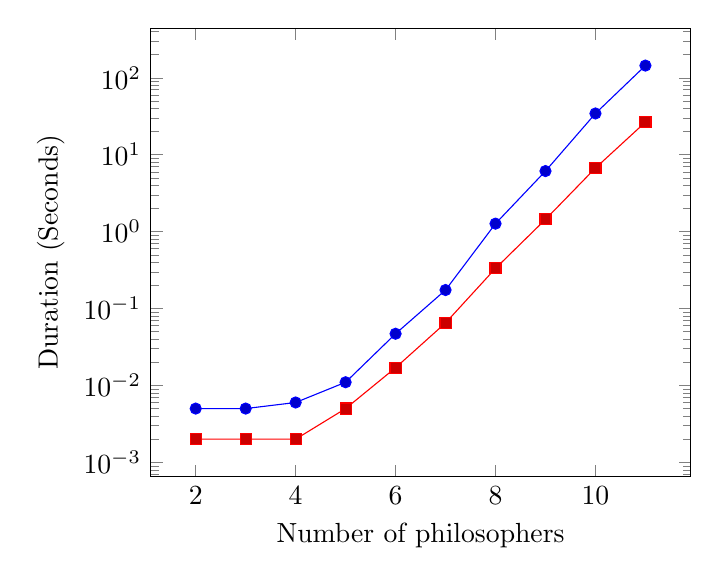
\begin{tikzpicture}
  	\begin{axis}[ 
    	xlabel={Number of philosophers},
    	ylabel={Duration (Seconds)},
    	ymode=log,
        log basis y={10}
  	] 
    \addplot+ [color=blue] coordinates {(2, 0.005) (3, 0.005) (4, 0.006) (5, 0.011) (6, 0.047) (7, 0.174) (8, 1.270) (9, 6.131) (10, 34.391) (11, 144.252)}; 
    
    \addplot+ [color=red] coordinates {(2, 0.002) (3, 0.002) (4, 0.002) (5, 0.005) (6, 0.017) (7, 0.065) (8, 0.333) (9, 1.442) (10, 6.716) (11, 26.529)}; 
  	\end{axis}
\end{tikzpicture}

\subsubsection{In every state, reachable by Plato not eating, Plato has the chance to starve}
This can be expressed with the formula:

\begin{center}
	{\tt nu X. (([i]X \&\& [others]X) \&\& nu Y. (<i>Y || <others>Y))}
\end{center}

The part {\tt nu X. (([i]X \&\& [others]X) ..)} iterates over all successor states as long as Plato does not eat, getting to each reachable state where Plato has not eaten yet. The other part states that for each of these states it must hold that there must exist an infinite sequence of states ({\tt \&\& nu Y.}) where Plato will not eat ({\tt (<i>Y || <others>Y)}).

The depths of this formula are: $ND = 2$, $AD = 1$ and $DAD = 1$.

This formula does not hold for all numbers of philosophers. See the graph below for the timings.

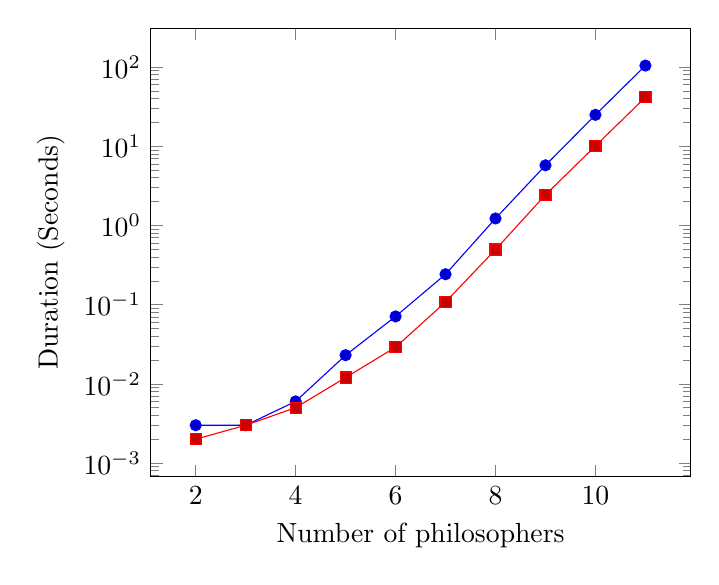
\begin{tikzpicture}
  	\begin{axis}[ 
    	xlabel={Number of philosophers},
    	ylabel={Duration (Seconds)},
    	ymode=log,
        log basis y={10}
  	] 
    \addplot+ [color=blue] coordinates {(2, 0.003) (3, 0.003) (4, 0.006) (5, 0.023) (6, 0.071) (7, 0.242) (8, 1.225) (9, 5.745) (10, 24.924) (11, 104.356)}; 
    
    \addplot+ [color=red] coordinates {(2, 0.002) (3, 0.003) (4, 0.005) (5, 0.012) (6, 0.029) (7, 0.108) (8, 0.496) (9, 2.435) (10, 10.081) (11, 41.595)}; 
  	\end{axis}
\end{tikzpicture}

\subsubsection{Invariantly, Plato can eat in some future}
This can be expressed with the formula:

\begin{center}
	{\tt nu X. (([i]X \&\& ([plato]X \&\& [others]X)) \&\& mu Y. ((<i>Y || <others>Y) || <plato>true ))}
\end{center}

The part {\tt nu X. (([i]X \&\& ([plato]X \&\& [others]X)) ..)} iterates over all successor states, getting to each reachable state. The other part states that from each of these states there must exist a finite sequence of states where Plato does not eat ({\tt \&\& mu Y. ((<i>Y || <others>Y) ..)} after which Plato will be able to eat ({\tt || <plato>true}).

The depths of this formula are: $ND = 2$, $AD = 2$ and $DAD = 1$.

This formula does not hold for all numbers of philosophers. See the graph below for the timings.

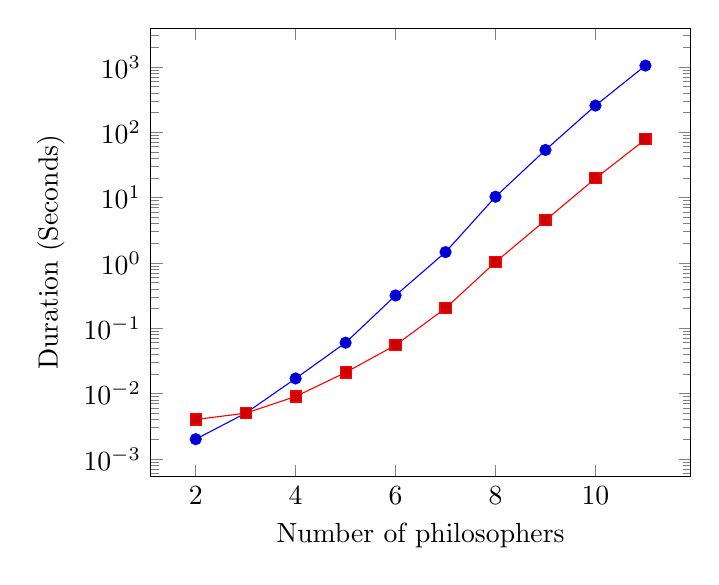
\begin{tikzpicture}
  	\begin{axis}[ 
    	xlabel={Number of philosophers},
    	ylabel={Duration (Seconds)},
    	ymode=log,
        log basis y={10}
  	] 
    \addplot+ [color=blue] coordinates {(2, 0.002) (3, 0.005) (4, 0.017) (5, 0.060) (6, 0.317) (7, 1.460) (8, 10.281) (9, 53.395) (10, 255.15) (11, 1044.492)}; 
    
    \addplot+ [color=red] coordinates {(2, 0.004) (3, 0.005) (4, 0.009) (5, 0.021) (6, 0.055) (7, 0.202) (8, 1.027) (9, 4.492) (10, 19.628) (11, 77.475)}; 
  	\end{axis}
\end{tikzpicture}

\subsubsection{There is a course of events in which Plato infinitely often eats}
This can be expressed with the formula:\\
{\tt nu X. mu Y. ((<plato>X || <i>Y) || <others>Y)}\\
The part {\tt mu Y. ((<plato>X || <i>Y) || <others>Y)} states that there must be a finite sequence of states where Plato does not eat, after which Plato will be able to eat. The part {\tt nu X. .. ((<plato>X ..) ..)} states that this sequence must be able to repeat itself infinitely often.\\
The depths of this formula are: $ND = 2$, $AD = 2$ and $DAD = 2$.\\
This formula holds for all numbers of philosophers. See the graph below for the timings.\\
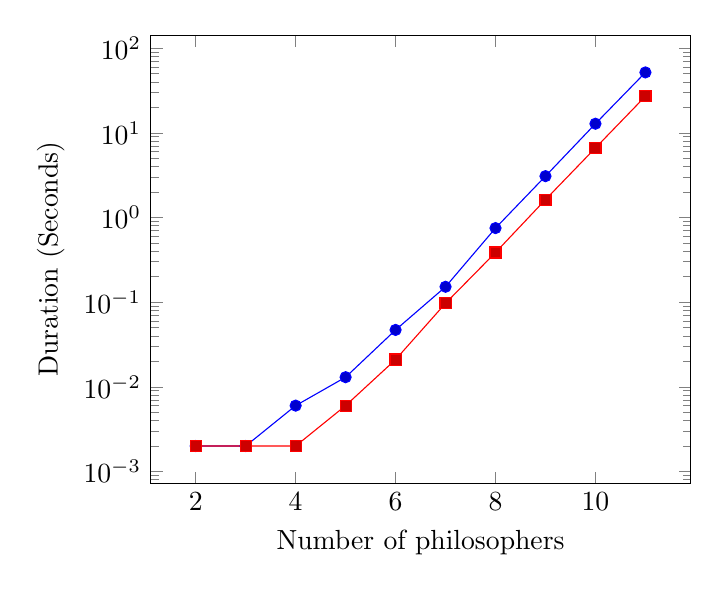
\begin{tikzpicture}
  	\begin{axis}[ 
    	xlabel={Number of philosophers},
    	ylabel={Duration (Seconds)},
    	ymode=log,
        log basis y={10}
  	] 
    \addplot+ [color=blue] coordinates {(2, 0.002) (3, 0.002) (4, 0.006) (5, 0.013) (6, 0.047) (7, 0.152) (8, 0.750) (9, 3.079) (10, 12.810) (11, 51.706)}; 
    
    \addplot+ [color=red] coordinates {(2, 0.002) (3, 0.002) (4, 0.002) (5, 0.006) (6, 0.021) (7, 0.097) (8, 0.386) (9, 1.626) (10, 6.633) (11, 27.038)}; 
  	\end{axis}
\end{tikzpicture}


\subsection{Demanding children}
The second experiment is about children that are initially playing. A child can ask a question, get the answer and return to playing (in that order). Only for one child the actions are named, this child will simply be referred to as 'the child'. For this experiment four mu-calculus formulas were made which are elaborated on below.

The graphs below shows the time in seconds that the program runs using labelled transition systems from 2 up to 10 demanding children. In these graphs the blue line indicates the timing of the naive algorithm and red indicates the timing of the improved algorithm.

\subsubsection{It is possible for the child to never ask a question}
This can be expressed with the formula:

\begin{center}
	{\tt nu X. ([i]X \&\& nu Y. <i>Y)}
\end{center}	
	
The part {\tt nu X. ([i]X ..)} iterates over all successor states as long as the child does nothing, getting to each reachable state where the child has not asked any question. The other part {\tt \&\& nu Y. <i>Y} states that from each of these states there must be an infinite sequence of states where the child does nothing (asks no question).

The depths of this formula are: $ND = 2$, $AD = 1$ and $DAD = 1$.

This formula holds for all numbers of demanding children. See the graph below for the timings.

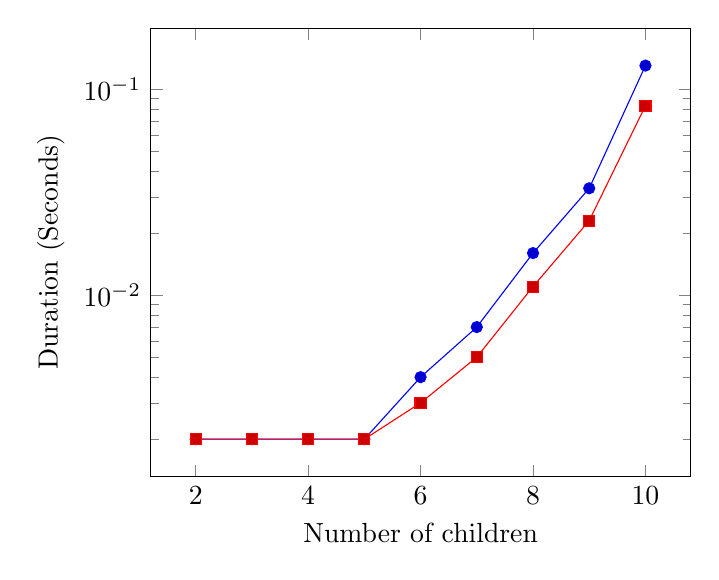
\begin{tikzpicture}
  	\begin{axis}[ 
    	xlabel={Number of children},
    	ylabel={Duration (Seconds)},
    	ymode=log,
        log basis y={10}
  	] 
    \addplot+ [color=blue] coordinates {(2, 0.002) (3, 0.002) (4, 0.002) (5, 0.002) (6, 0.004) (7, 0.007) (8, 0.016) (9, 0.033) (10, 0.130)}; 
    
    \addplot+ [color=red] coordinates {(2, 0.002) (3, 0.002) (4, 0.002) (5, 0.002) (6, 0.003) (7, 0.005) (8, 0.011) (9, 0.023) (10, 0.083)}; 
  	\end{axis}
\end{tikzpicture}

\subsubsection{It is possible for all other children to never ask a question}
This can be expressed with the formula:

\begin{center}
	{\tt nu X. ((([ask]X \&\& [wisdom]X) \&\& [playing]X) \&\& nu Y. ((<ask>Y || <wisdom>Y) || <playing>Y))}
\end{center}

The part {\tt nu X. ((([ask]X \&\& [wisdom]X) \&\& [playing]X)} iterates over all successor states as long as the other children than the child do nothing, getting to each reachable state where the other children than the child have not asked any question. The other part {\tt \&\& nu Y. ((<ask>Y || <wisdom>Y) || <playing>Y)} states that from each of these states there must be an infinite sequence of states where the other children than the child do nothing (ask no question).

The depths of this formula are: $ND = 2$, $AD = 1$ and $DAD = 1$.

This formula holds for all numbers of demanding children. See the graph below for the timings.

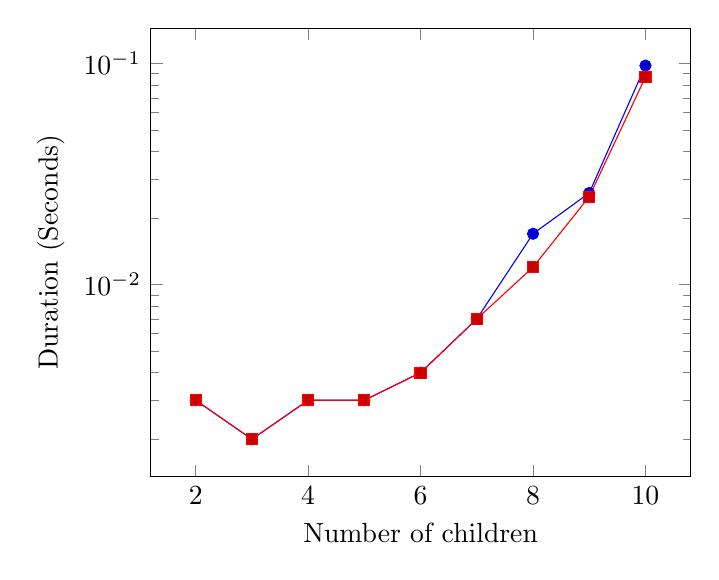
\begin{tikzpicture}
  	\begin{axis}[ 
    	xlabel={Number of children},
    	ylabel={Duration (Seconds)},
    	ymode=log,
        log basis y={10}
  	] 
    \addplot+ [color=blue] coordinates {(2, 0.003) (3, 0.002) (4, 0.003) (5, 0.003) (6, 0.004) (7, 0.007) (8, 0.017) (9, 0.026) (10, 0.098)}; 
    
    \addplot+ [color=red] coordinates {(2, 0.003) (3, 0.002) (4, 0.003) (5, 0.003) (6, 0.004) (7, 0.007) (8, 0.012) (9, 0.025) (10, 0.087)}; 
  	\end{axis}
\end{tikzpicture}

\subsubsection{If the child asks his/her first question the child will eventually be answered}
This can be expressed with the formula:

\begin{center}
	{\tt nu X. ([i]X \&\& <ask>mu Y. ([i]Y \&\& <wisdom>true))}
\end{center}	
	
The part {\tt nu X. ([i]X ..)} iterates over all successor states as long as the child does nothing, getting to each reachable state where the child has not asked any question. The other part states that from each of these states it must be possible to ask a question ({\tt \&\& <ask>}) after which for every finite sequence of the child not being answered (not doing anything, {\tt mu Y. ([i]Y ..)}) the child will be answered afterwards ({\tt \&\& <wisdom>true}).

The depths of this formula are: $ND = 2$, $AD = 2$ and $DAD = 1$.

This formula does not hold for all numbers of demanding children. See the graph below for the timings.

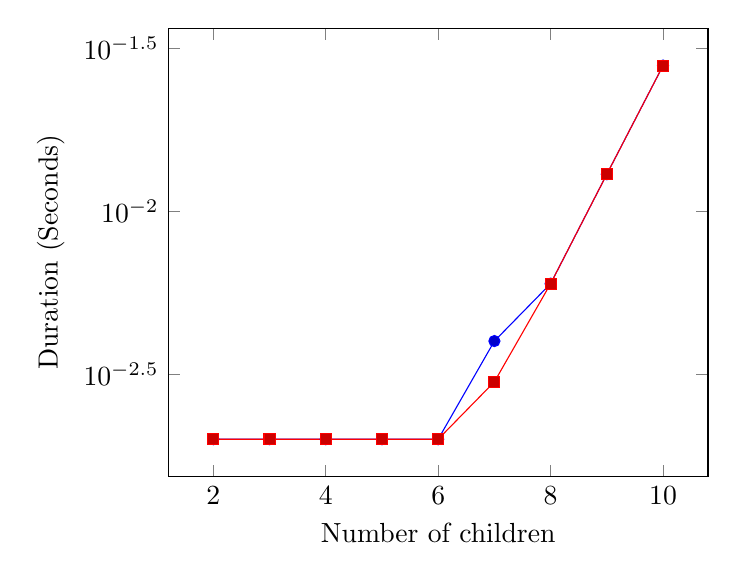
\begin{tikzpicture}
  	\begin{axis}[ 
    	xlabel={Number of children},
    	ylabel={Duration (Seconds)},
    	ymode=log,
        log basis y={10}
  	] 
    \addplot+ [color=blue] coordinates {(2, 0.002) (3, 0.002) (4, 0.002) (5, 0.002) (6, 0.002) (7, 0.004) (8, 0.006) (9, 0.013) (10, 0.028)}; 
    
    \addplot+ [color=red] coordinates {(2, 0.002) (3, 0.002) (4, 0.002) (5, 0.002) (6, 0.002) (7, 0.003) (8, 0.006) (9, 0.013) (10, 0.028)}; 
  	\end{axis}
\end{tikzpicture}

\subsubsection{There is a course of events where the child can ask an infinite number of questions}
This can be expressed with the formula:

\begin{center}
	{\tt nu X. mu Y. (((<ask>X || <i>Y) || <wisdom>Y) || <playing>Y)}
\end{center}	
	
The part {\tt mu Y. (((<ask>X || <i>Y) || <wisdom>Y) || <playing>Y)} states that there must be a finite sequence of states where the child does not ask a question, after which the child will be able to ask a question. The part {\tt nu X. .. (((<ask>X ..) ..) ..)} states that this sequence must be able to repeat itself infinitely often.

The depths of this formula are: $ND = 2$, $AD = 2$ and $DAD = 2$.

This formula holds for all numbers of demanding children. See the graph below for the timings.

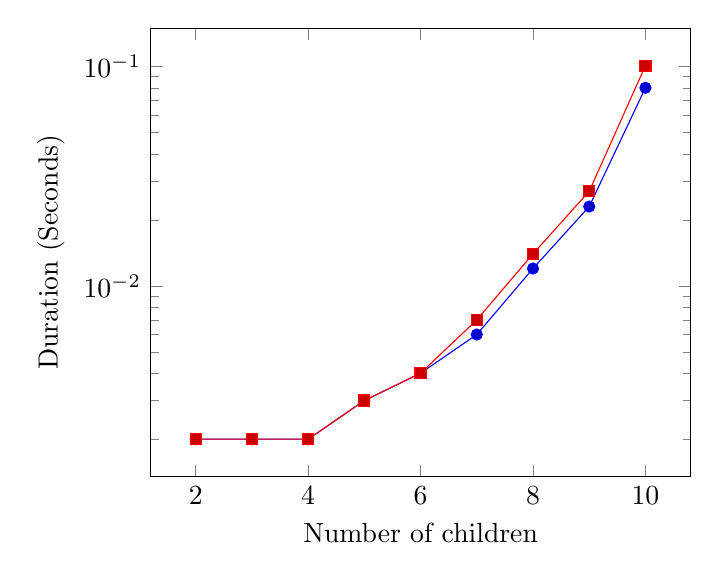
\begin{tikzpicture}
  	\begin{axis}[ 
    	xlabel={Number of children},
    	ylabel={Duration (Seconds)},
    	ymode=log,
        log basis y={10}
  	] 
    \addplot+ [color=blue] coordinates {(2, 0.002) (3, 0.002) (4, 0.002) (5, 0.003) (6, 0.004) (7, 0.006) (8, 0.012) (9, 0.023) (10, 0.080)}; 
    
    \addplot+ [color=red] coordinates {(2, 0.002) (3, 0.002) (4, 0.002) (5, 0.003) (6, 0.004) (7, 0.007) (8, 0.014) (9, 0.027) (10, 0.101)}; 
  	\end{axis}
\end{tikzpicture}


\subsection{Boardgame}
The third and last experiment is about two players playing a board game. The game is played on a $N$ by $N$ board and they start at state $(0, 0)$. Each player alternatively can choose to make a move, starting with player I. Player II wins whenever the game reaches state $(N, N)$. In the LTS being in the state $(N, N)$ is denoted by being able to do the transition {\tt won}. For this experiment three mu-calculus formulas are made which are elaborated on below.

The graphs below shows the time in seconds that the program runs using labelled transition systems for $N \in \{50, 100, 150, 200, 250, 300, 350, 400, 450, 500\}$. In these graphs the blue line indicates the timing of the naive algorithm and red indicates the timing of the improved algorithm.

\subsubsection{3a) There is a play such that player II can win}
This can be expressed with the formula:

\begin{center}
	{\tt mu X. (<choose1><choose2>X || <won>true)}
\end{center}	
	
This formula states that there must be a finite sequence of states in which first player I makes a choice and then player II ({\tt mu X. (<choose1><choose2>X ..)}) after which the game will end up in state $(N, N)$, causing player II to win ({\tt || <won>true}).

The depths of this formula are: $ND = 1$, $AD = 1$ and $DAD = 1$.

This formula holds for all numbers of $N$, except for $N = 350$. See the graph below for the timings.

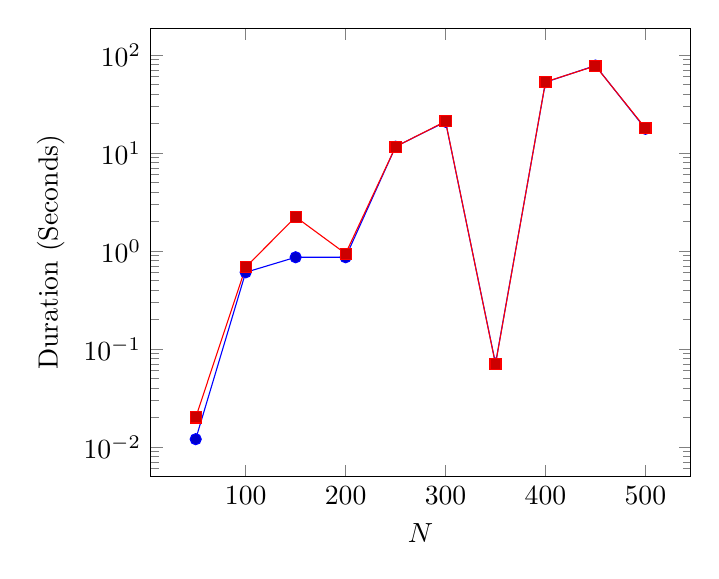
\begin{tikzpicture}
  	\begin{axis}[ 
    	xlabel={$N$},
    	ylabel={Duration (Seconds)},
    	ymode=log,
        log basis y={10}
  	] 
    \addplot+ [color=blue] coordinates {(50, 0.012) (100, 0.605) (150, 0.862) (200, 0.862) (250, 11.583) (300, 20.812) (350, 0.071) (400, 52.675) (450, 77.872) (500, 17.618)}; 
    
    \addplot+ [color=red] coordinates {(50, 0.020) (100, 0.682) (150, 2.225) (200, 0.939) (250, 11.580) (300, 20.989) (350, 0.070) (400, 53.083) (450, 77.293) (500, 17.920)}; 
  	\end{axis}
\end{tikzpicture}

\subsubsection{3b) Player II wins the game}\label{board2}
This can be expressed with the formula:

\begin{center}
	{\tt mu X. ([choose1]<choose2>X || <won>true)}
\end{center}	
	
This formula states that whatever move player I chooses ({\tt [choose1]}) player II can choose a move (player II has a strategy, {\tt <choose2>}) such that the game will have a finite sequence of states ({\tt mu X. ([choose1]<choose2>X ..)}) such that the game ends up in state $(N, N)$, causing player II to win ({\tt || <won>true}).

The depths of this formula are: $ND = 1$, $AD = 1$ and $DAD = 1$.

The formula holds for all numbers of $N$, except for $N \in \{50, 200, 350, 500\}$. See the graph below for the timings.

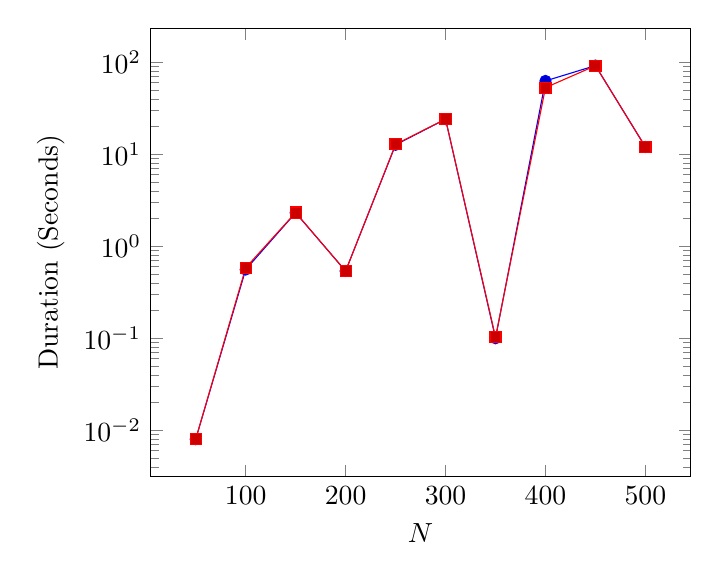
\begin{tikzpicture}
  	\begin{axis}[ 
    	xlabel={$N$},
    	ylabel={Duration (Seconds)},
    	ymode=log,
        log basis y={10}
  	] 
    \addplot+ [color=blue] coordinates {(50, 0.008) (100, 0.559) (150, 2.318) (200, 0.539) (250, 12.693) (300, 24.134) (350, 0.100) (400, 62.880) (450, 92.274) (500, 12.03)}; 
    
    \addplot+ [color=red] coordinates {(50, 0.008) (100, 0.584) (150, 2.329) (200, 0.537) (250, 12.840) (300, 24.197) (350, 0.103) (400, 53.143) (450, 91.960) (500, 12.036)}; 
  	\end{axis}
\end{tikzpicture}

\subsubsection{3c) Player II wins the game by being able to move the token to place (N, N) infinitely often}\label{board3}
This can be expressed with the formula:

\begin{center}
	{\tt nu Y. mu X. ([choose1]<choose2>X || ([choose1]<choose2><won>true \&\& [choose1]<choose2>Y))}
\end{center}

The part {\tt mu X. ([choose1]<choose2>X ..)} states that there must be a finite sequence of states in which player I chooses any step and player II does a certain step (according to a strategy). The other part says that after this finite sequence player II will be able to move to state $(N, N)$ within a turn independent of what player I does ({\tt || ([choose1]<choose2><won>true ..)}) and after one turn it is possible to repeat this sequence ({\tt nu Y. .. (.. (.. \&\& [choose1]<choose2>Y))}), causing the game to get to state $(N, N)$ infinitely often, causing player II to win.

The depths of this formula are: $ND = 2$, $AD = 2$ and $DAD = 2$.

This formula holds for all numbers of $N$, except for $N \in \{50, 200, 350, 500\}$. See the graph below for the timings.

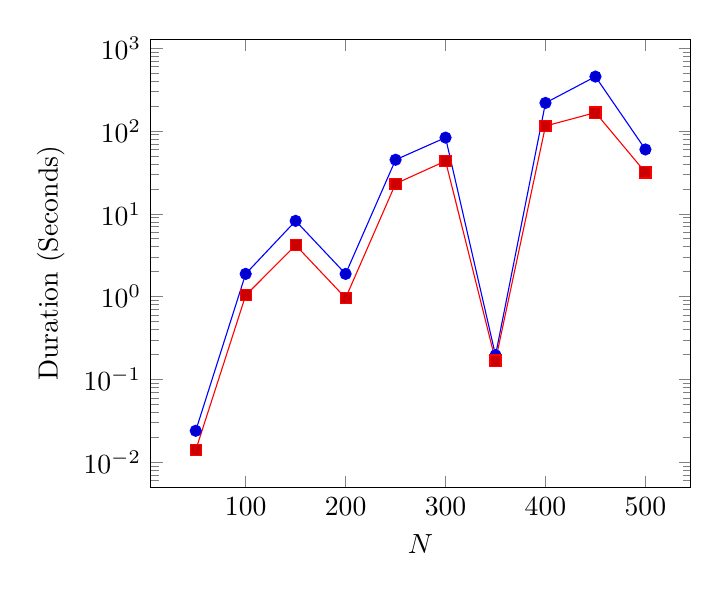
\begin{tikzpicture}
  	\begin{axis}[ 
    	xlabel={$N$},
    	ylabel={Duration (Seconds)},
    	ymode=log,
        log basis y={10}
  	] 
    \addplot+ [color=blue] coordinates {(50, 0.024) (100, 1.883) (150, 8.219) (200, 1.881) (250, 44.914) (300, 83.155) (350, 0.196) (400, 218.213) (450, 453.711) (500, 59.833)}; 
    
    \addplot+ [color=red] coordinates {(50, 0.014) (100, 1.036) (150, 4.183) (200, 0.962) (250, 23.098) (300, 43.393) (350, 0.169) (400, 114.784) (450, 166.791) (500, 31.597)}; 
  	\end{axis}
\end{tikzpicture}


\section{Conclusion}\label{conc}

\subsection{Correctness}
Our implemented algorithms are able to give the correct answer for checking whether a modal mu-calculus formula holds for a given labelled transition system. This is verified by running the same experiments using the mCRL2 toolset (version 201409.1.13211) \cite{mcrl2}.


\subsection{Performance}
In most cases with multiple alternating fixed points the Emerson-Lei algorithm does perform better than the naive algorithm as expected. In most other cases the Emerson-Lei algorithm does either perform better than or about equal to the naive algorithm.\\ However, especially in the cases that the algorithm needs very little time the Emerson-Lei version is sometimes slower than the naive algorithm. This is likely due to the overhead generated by the extra tasks this version does such as the initialisation.\\
The boardgame experiment resulted in timings that were not always increasing for bigger $N$. For the cases $N \in \{50, 200, 350, 500\}$ the timing seems lower than expected. These are also the cases where the solver returns false for formulas \ref{board2} and \ref{board3}. Since mCRL2 gives the same solver results and shows the same timing behaviour, we suspect that these anomalies are caused by the strong bisimulation reduction applied to the labelled transition systems.




\begin{thebibliography}{9}
	\bibitem{aldebaran} \url{http://www.mcrl2.org/dev/user_manual/language_reference/lts.html#aldebaran-format}
	
	\bibitem{muparse} \url{http://www.win.tue.nl/\~timw/downloads/parser.pdf}

	\bibitem{mcrl2} \url{http://www.mcrl2.org/}
	
\end{thebibliography}

\end{document}